\documentclass{beamer}
\usepackage{amsmath}
\usepackage{graphicx}
\usetheme{Copenhagen}
\usecolortheme[named=red]{structure}

\author{Castleberry, Cherry, and Firth}
\title{Efficient Stop \& Warning Sign and Pedestrian Detection}
\date{\today}

\begin{document}
\maketitle

\section{Introduction and Overview}
\frame{ \frametitle{Overview}
 \begin{itemize}
   \item We implemented the following:
   \begin{itemize}
    \item Stop-sign detector, using the notion of integral
          images from SURF
    \item Warning sign detector, using perspective transformation
          on a model image, then SURF 
   \end{itemize} 
 \end{itemize} 
}

\frame{ \frametitle{Wrappers}
 \begin{itemize} 
  \item We created a wrapper to the pedestrian detector to gain
        familiarity with the EmguCV library.
  \item We also created a wrapper to the built-in EmguCV SURF detector
        to use as a basis of comparison for our own methods.
 \end{itemize} 
}

\frame{ \frametitle{} \includegraphics[width=\textwidth]{uml.png} }

\section{Stop Signs}

\frame{ \frametitle{} 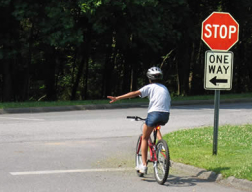
\includegraphics[width=\textwidth]{pos-stop.jpg} }
\frame{ \frametitle{} 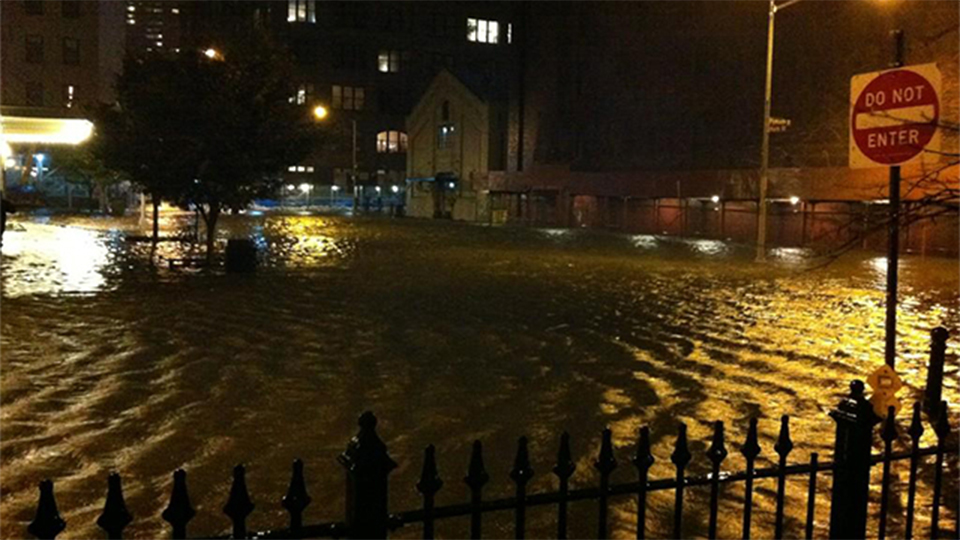
\includegraphics[width=\textwidth]{neg-stop.jpg} }

\frame{ \frametitle{Stop Sign Detection, Integral Images}
 \begin{itemize} 
  \item We developed a method for detecting stop signs based upon
        the use of integral images which we encountered in the
        SURF algorithm.
  \item To summarize the method, we use integral images from both
        the left-hand side (top left) and the right-hand side
        (bottom right) on only the R channel. Then we consider only 
        the LHS and RHS
        integral images along the diagonal of the image.  We
        difference these, then fit a Gaussian curve to the
        resulting vector.  We threshold the curve at the points
        of inflection to generate a bounding box for the sign.
 \end{itemize} 
}

\frame{ \frametitle{} 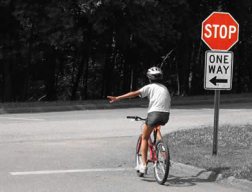
\includegraphics[width=\textwidth]{pos-stop-red.jpg} }

\frame{ \frametitle{Stop Sign Detection, Integral Images}
 \begin{itemize} 
  \item To begin our method, we scale the $N \times M$ image
        to $N \times N$ for $N<M$, $M \times M$ for $M<N$.  We
        require a square matrix to extract a particular vector.
  \item Recall that the formula for computing the integral image
        $\mathcal{I_{-}}$ at a pixel $(x, y)$ with intensity value
        $I(x,y)$ is:
  \begin{equation}
   \mathcal{I}_{-}(x,y) = \sum_{i=0}^{n_x} \sum_{j=0}^{n_y} I(x,y)
  \end{equation}
  \item We compute the integral image at a pixel using the following formula:
  \begin{equation}
   \mathcal{I}_{x,y} = \mathcal{I}_{x-1,y}+ \mathcal{I}_{x,y-1}- \mathcal{I}_{x-1,y-1}
  \end{equation}
 \end{itemize} 
}

\frame{ \frametitle{} 
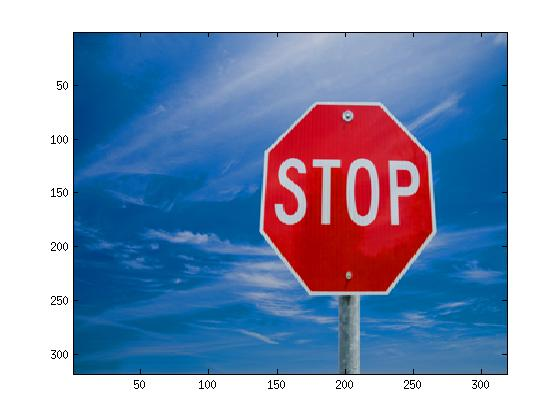
\includegraphics[width=.9\textwidth]{test-sign.jpg} }

\frame{ \frametitle{Stop Sign Detection, Integral Images}
 \begin{itemize} 
  \item Likewise, we compute an RHS integral image 
        $\mathcal{I_{+}}$ at a pixel $(x, y)$ with intensity value
        $I(x,y)$ as:
  \begin{equation}
   \mathcal{I}_{+}(x,y) = \sum_{i=N}^{n_x} \sum_{j=N}^{n_y} I(x,y)
  \end{equation}
 \end{itemize} 
}

\frame{ \frametitle{} 
\begin{center}
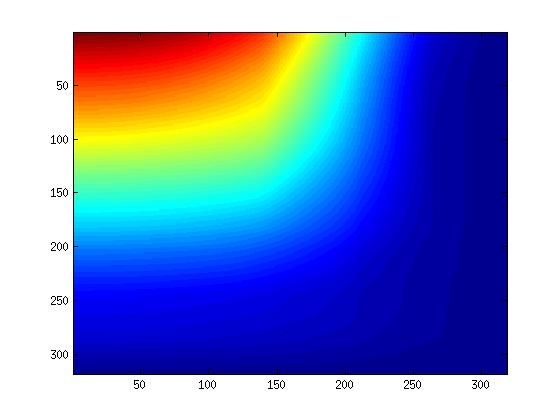
\includegraphics[width=.4\textwidth]{rhs.jpg} 
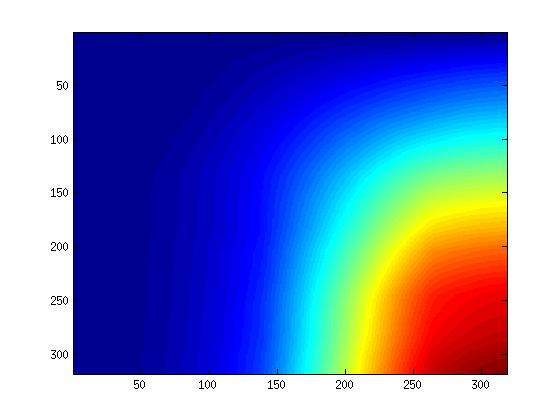
\includegraphics[width=.4\textwidth]{lhs.jpg} 
\end{center}
}

\frame{ \frametitle{Stop Sign Detection, Integral Images}
 \begin{itemize} 
  \item After obtaining the integral image, we copy its diagonal
        into a vector $u$.
  \item We then apply a finite-difference method to the elements in
        $u$ and store it in $v$, as follows:
  \begin{equation}
   v_{n} = u_{n} - u_{n-1}
  \end{equation}
  The vector $v$ gives the LHS crosshair of the R-channel. For images
  which have stop signs, $v$ has a Gauss distribution.
 \end{itemize} 
}

\frame{ \frametitle{Stop Sign Detection, Integral Images}
 \begin{itemize} 
  \item We apply this finite-difference method for both vectors
        $u_{-}$ and $u_{+}$ to obtain $v_{-}$ and $v_{+}$.
  \item Then, we add $v_{-}$ and $v_{+}$ to obtain a vector
        $m$.
  \item Finally, we compute the standard deviation $\sigma$ of
        the vector $m$ and its centroid $c$, then apply a Gaussian
        fit to the data in $m$.  We call the Gaussian fit $G$.
  \item We then apply finite-differencing to the Gaussian fit $G$
        to obtain $G'$, then find the indices at $min(G')$ and 
        $max(G')$.
  \item These indices form the bounding box for the image.
 \end{itemize} 
}

\frame{ \frametitle{} 
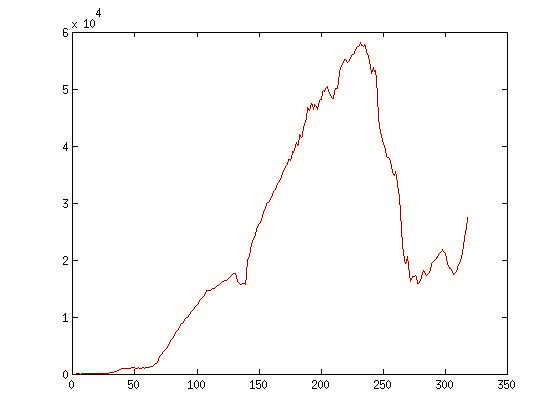
\includegraphics[width=.9\textwidth]{crosshair-curve.jpg} }

\frame{ \frametitle{} 
\begin{center}
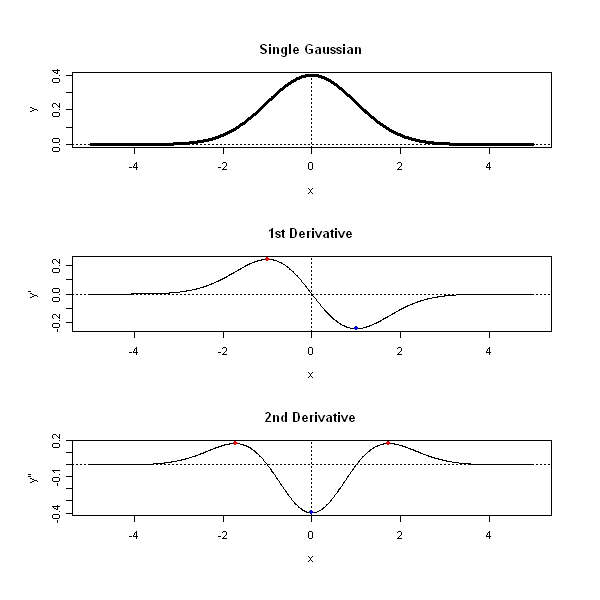
\includegraphics[width=.7\textwidth]{gaussian.png} 
\end{center} }

\section{Warning Signs}

\frame{ \frametitle{Warning Signs}
  \begin{itemize}
    \item For our warning sign detection, we experimented with 
          SURF in combination with perspective transformations
          on out-of-plane-rotated signs. 
    \item In particular, we assume that we know the perspective
          information of an out-of-plane-rotated sign.  We apply
          a perspective transform to a model sign, then apply
          SURF to the two images, then match.
  \end{itemize} 
}

\frame{ \frametitle{} 
\begin{center}
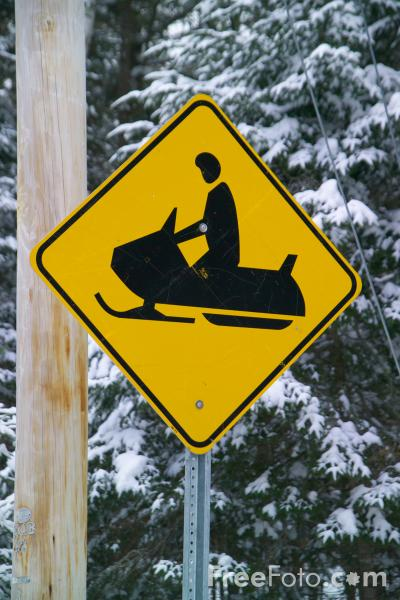
\includegraphics[width=.5\textwidth]{pos-warning.jpg} 
\end{center} }

\frame{ \frametitle{Warning Signs}
  \begin{itemize}
    \item We first hand-annotated $N$ images using a MATLAB code.
    \item From this, we extracted a set of $4N$ points which
          give the vertices of the warning sign.  We then applied
          \texttt{getPerspectiveTransform()} on the points, which
          returns a perspective transform matrix \texttt{M}.
    \item We apply this perspective transform matrix to the model
          with the function \texttt{warpPerspective()}.
    \item We then run SURF on the two images, then compare their
          feature descriptors to obtain a match within a threshold
          of $t_\epsilon$.
  \end{itemize} 
}

\frame{ \frametitle{Perspective Transform}
  \begin{itemize}
    \item If $a_{x,y,z}$ is the point to be projected, $c_{x,y,z}$ 
          is the camera, $\theta_{x,y,z}$ is the camera orientation and
          $e_{x,y,z}$ is the position of the viewer relative to the 
          display surface then $b_{x,y}$, the 2D projection of $a$, is 
          given by:
\tiny
\begin{equation}
\begin{bmatrix} d_x \\ d_y \\ d_z \end{bmatrix} =
\begin{bmatrix}
                1   &  0   &  0 \\
                0   &  cos(\theta_x) &  -sin(\theta_x) \\ 
                0   &  sin(\theta_x) &  cos(\theta_x)  
\end{bmatrix}
\begin{bmatrix}
                cos(\theta_y) & 0 & sin(\theta_y) \\ 
                0   &  1   &  0 \\
               -sin(\theta_y) & 0 & cos(\theta_y) 
\end{bmatrix}
\begin{bmatrix}
                cos(\theta_z) &  -sin(\theta_z) & 0 \\ 
                sin(\theta_z) &  cos(\theta_z)  & 0 \\ 
                0   &  0   &  1 
\end{bmatrix}
(
\begin{bmatrix} a_x \\ a_y \\ a_z \end{bmatrix} -
\begin{bmatrix} c_x \\ c_y \\ c_z \end{bmatrix}
).
\end{equation}
\normalsize
    \item A visual example follows.
  \end{itemize} 
}

\frame{ \frametitle{} 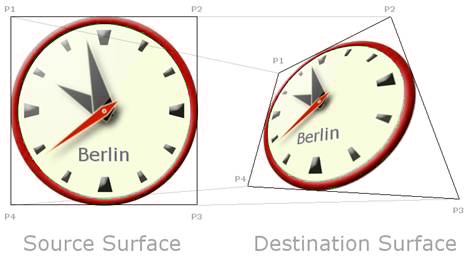
\includegraphics[width=\textwidth]{perspective.jpg} }

\section{Results and Conclusion}

\frame{ \frametitle{Results}
  \begin{itemize}
    \item We considered there to be a match if at least
          50\% of the sign fell within the area of the
          bounding box. 
    \item The following table summarizes our results:
  \end{itemize} 
  \vspace{8pt}
  \begin{tabular}{lc}
  Surf Stop Sign Detector             & 17\% \\
  Integral Images Stop Sign Detector  & 67\% \\ 
  Surf Warning Sign Detector          & 42\% \\
  Oriented Surf Warning Sign Detector & 62\% \\
  \end{tabular}
  \vspace{8pt}
  \begin{itemize}
    \item As is evident in the above, our accuracy for \ldots was an 
    abysmal $N\%$.
  \end{itemize} 
}

\frame{ \frametitle{Conclusion}
 \begin{itemize}
  \item Bearing in mind that the accuracy for our integral image 
        detector was much less than the accuracy for the built-in 
        SURF algorithm, we conclude that in the development of
        computer vision algorithms, one should:
  \begin{enumerate}
   \item Not over-utilize heuristics, and 
   \item Develop the algorithm starting from optimized versions
         of existing algorithms.
  \end{enumerate} 
 \end{itemize} 
}

\end{document}
